\documentclass[12pt]{article}
\usepackage{styles/cwilliams-standard}

% Set up document metadata
\setauthors{Tzu-Chen Chiu, Arjun Sivakumar, Mara Schimmel, Christopher Williams}
\setheaderauthors{Chiu, Sivakumar, Schimmel, Williams}
\settitle{Sprint 2 Report}
\setclass{IPD}

\begin{document}

\maketitlepage

\begin{important}{Sprint 3 Progress}
    This sprint was a lackluster sprint for our group because deadlines and requirements for 
    other classes including assignments, projects, and exams. We apologize for this performance 
    and will make doubly sure to cover the lost ground in the next sprint. 
\end{important}

\section{Original Sprint 3 Backlog}

\begin{figure}[H]
    \centering
    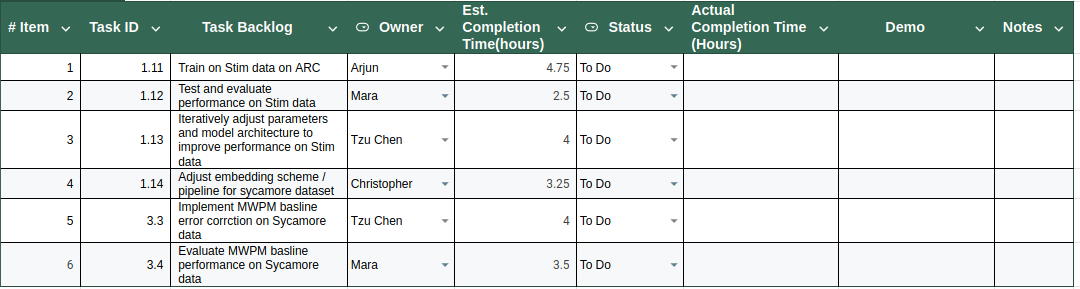
\includegraphics[width=1\textwidth]{images/sprint3_backlog.png}
    \caption{Spring 3 Backlog}
\end{figure}

\section{Sprint 3 Backlog - End of Sprint Status}

\begin{figure}[H]
    \centering
    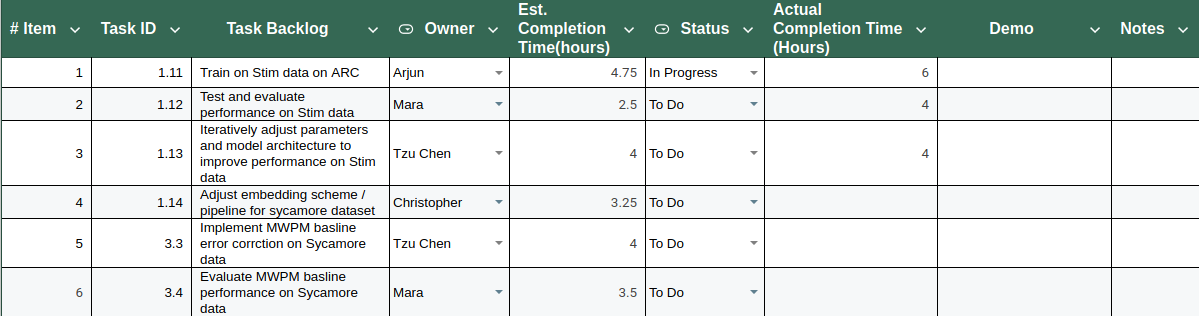
\includegraphics[width=1\textwidth]{images/sprint_3_updated.png}
    \caption{Spring 3 Backlog - Updated}
    \label{fig:sprint3updated}
\end{figure}

\section{Project Management Screenshots}

The Sprint backlogs in Google Sheets are being used to manage tasks.

\section{Sprint Retrospective}

\subsection*{Mara}

\subsection*{Chris}

This sprint was particularly lack luster in terms of progress and overall accomplishment because of 
many deadlines and responsibilites in other classes. I am aware that this is not an acceptable mindset 
or outcome, especially for working life. The reason I made the decision to tackle my sprint objectives 
next sprint is in the fact that there is another sprint. The design of this project allows for us to 
shift goals and deliverables around and the extension of this class track into two semesters presents an 
opportunity like I had this semester to prioritize shorter term requirements and to look long term at what 
I will have time to accomplish next semester.

\subsection*{Tzu-Chen}

\subsection*{Arjun}

\section{Product Backlog (Updated)}

\begin{figure}[H]
    \centering
    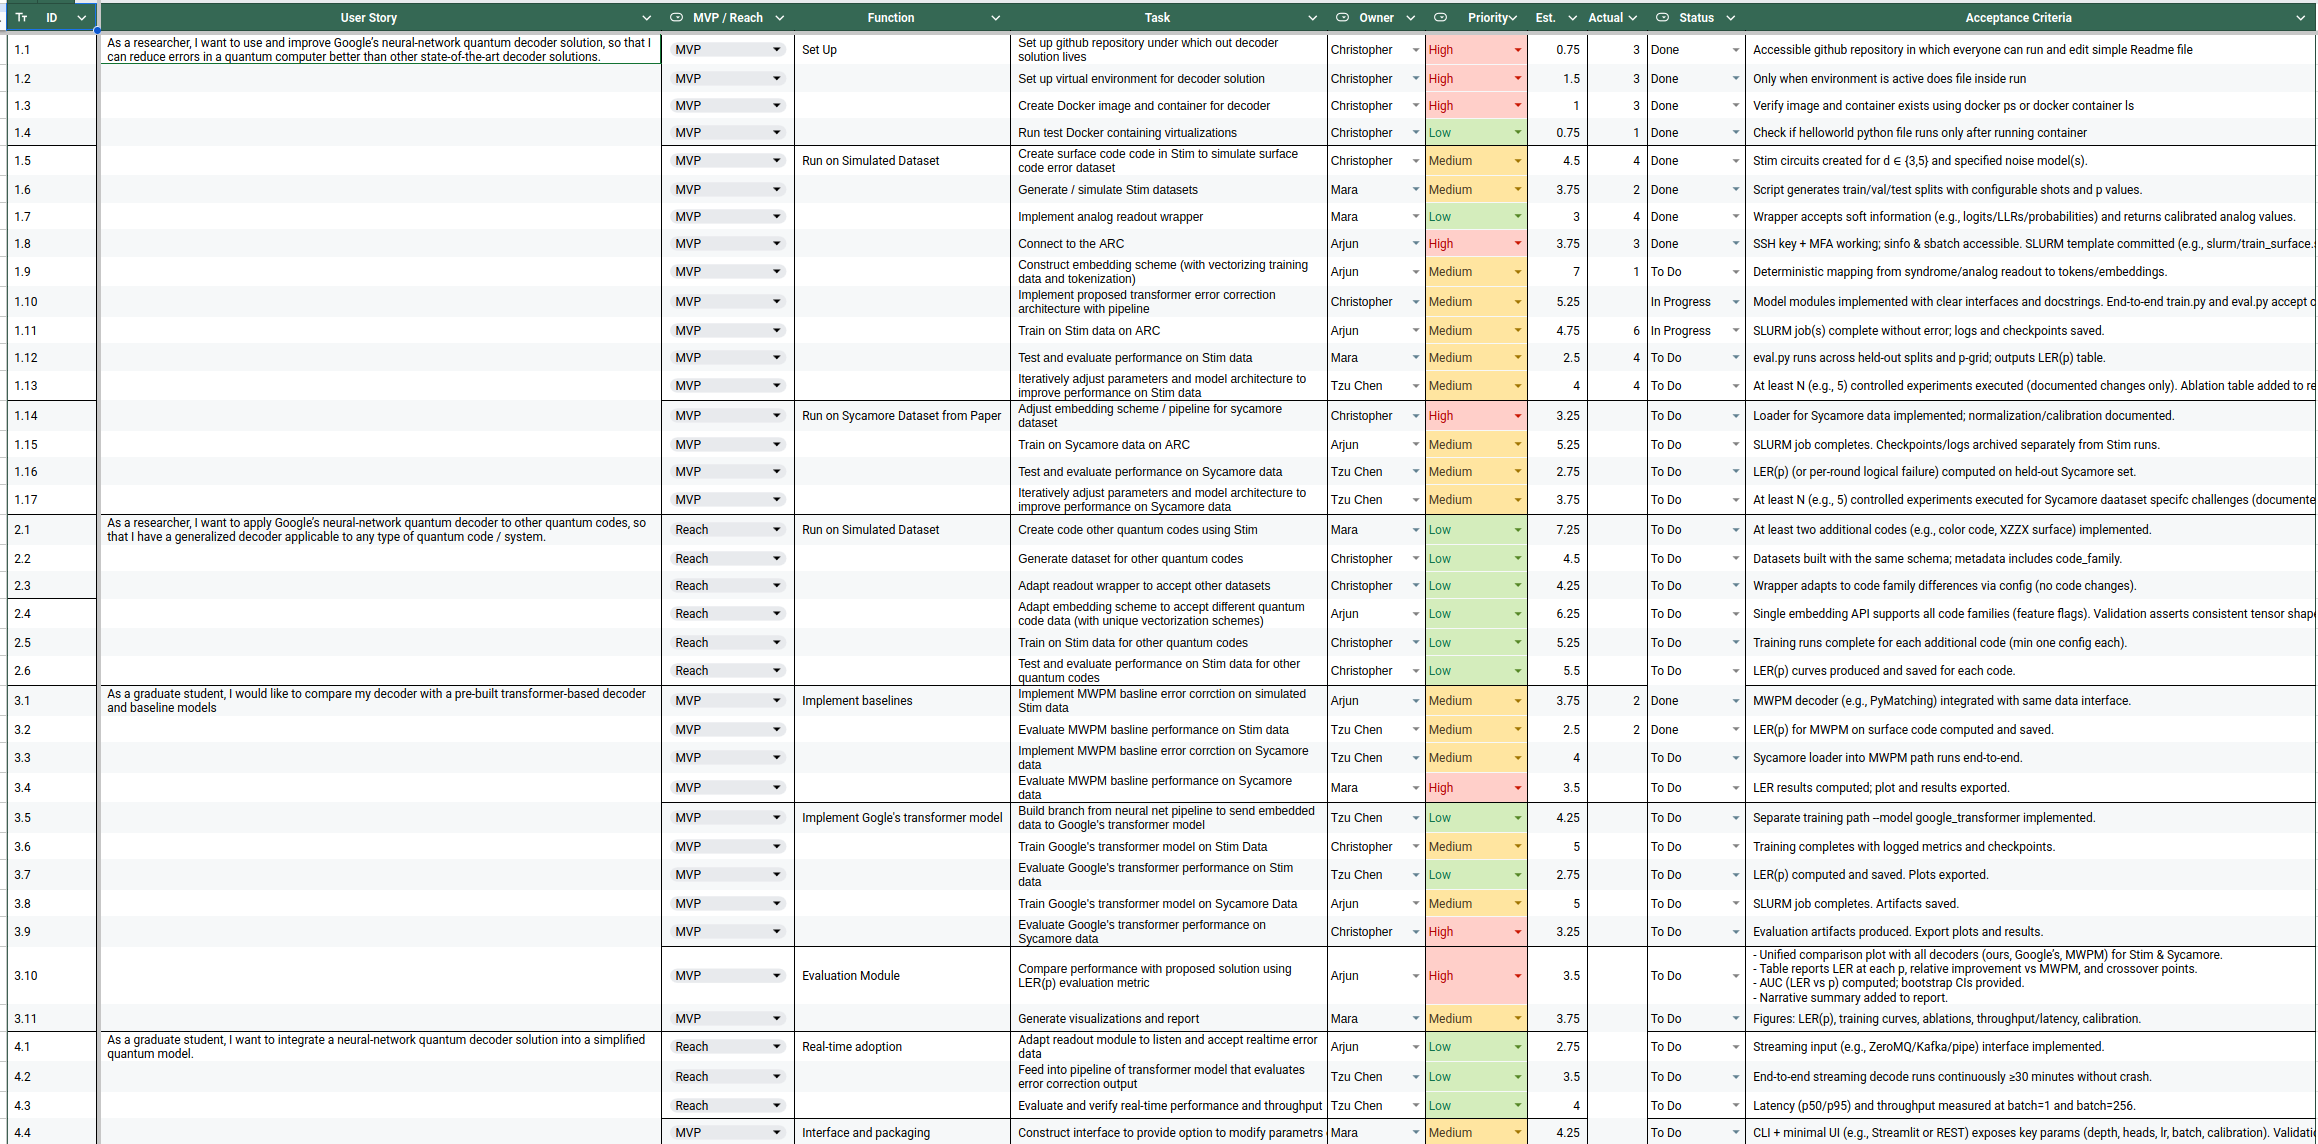
\includegraphics[width=1\textwidth]{images/sprint3_updated_product_backlog.png}
    \caption{Updated Product Backlog}
\end{figure}

\begin{aside}{Picture Quality}
    We understand that this image is hard to read, but as Figure \ref{fig:sprint3updated} shows, tasks 
    1.11 was worked on.
\end{aside}

\section{Issue Tracking}

\begin{table}[H]
\centering
\begin{tabular}{@{}llll@{}}
\toprule
\textbf{Issue} & \textbf{Description} & \textbf{Status} & \textbf{Date Completed} \\ \midrule
ARC Access & Getting every member access to the ARC & 12/9/2025 \\
Train on Stim Data & Getting reasonable results in training & Ongoing \\
\end{tabular}
\caption{Issue Tracking Summary}
\end{table}

\section{Sprint 4 Backlog}

\begin{figure}[H]
    \centering
    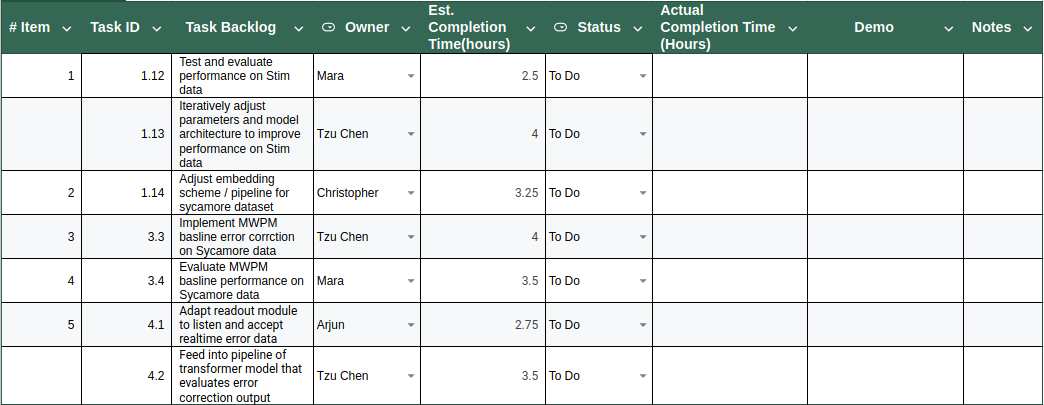
\includegraphics[width=1\textwidth]{images/sprint_4_backlog.png}
    \caption{Spring 4 Backlog}
\end{figure}

\section{Member Videos}

Members that did not have progress for this week do not have demo videos to submit.

\end{document}